\documentclass[12pt,a4paper]{article}
\usepackage{amsmath}
\usepackage{mdframed}
\usepackage{graphicx}

\begin{document}
	
% Folha de rosto
\begin{titlepage}
	\centering
	\vspace{2cm}
	
	{UNIVERSIDADE FEDERAL FLUMINENSE} \\ [0.1cm]
	{BACHARELADO EM CIÊNCIA DA COMPUTAÇÃO} \\ [0.1cm]
	{TCC00297 - INTELIGÊNCIA ARTIFICIAL}
	
	\vfill
	
	{\Large \bfseries Trabalho de Classificação}
	
	\vfill
	
	{BEATRIZ DE OLIVEIRA PIEDADE}
	
	\vfill
	{NITERÓI} \\
	{2024}
\end{titlepage}

\tableofcontents

\newpage
\section{Introdução} 

\quad\space O objetivo deste trabalho é realizar a classificação do conjunto de dados "Secondary Mushroom", buscando prever se um cogumelo é comestível ou venenoso. O dataset foi analisado com foco na preparação, construção e avaliação de modelos de Machine Learning que maximizem a performance em métricas relevantes.

O conjunto de dados contém 61.068 registros e 21 atributos. A tabela abaixo apresenta uma visão geral dos atributos disponíveis no conjunto:

\begin{table}[h]
	\centering
	\begin{tabular}{|l|l|l|l|}
		\hline
		\textbf{Nome} & \textbf{Papel} & \textbf{Tipo} & \textbf{ Valores ausentes} \\
		\hline
		class & Target & Categorical & no \\
		\hline
		cap-diameter & Feature & Continuous & no \\
		\hline
		cap-shape & Feature & Categorical & no \\
		\hline
		cap-surface & Feature & Categorical & yes \\
		\hline
		cap-color & Feature & Categorical & no \\
		\hline
		does-bruise-or-bleed & Feature & Categorical & no \\
		\hline
		gill-attachment & Feature & Categorical & yes \\
		\hline
		gill-spacing & Feature & Categorical & yes \\
		\hline
		gill-color & Feature & Categorical & no \\
		\hline
		stem-height & Feature & Continuous & no \\
		\hline
		stem-width & Feature & Continuous & no \\
		\hline
		stem-root & Feature & Categorical & yes \\
		\hline
		stem-surface & Feature & Categorical & yes \\
		\hline
		stem-color & Feature & Categorical & no \\
		\hline
		veil-type & Feature & Categorical & yes \\
		\hline
		veil-color & Feature & Categorical & yes \\
		\hline
		has-ring & Feature & Categorical & no \\
		\hline
		ring-type & Feature & Categorical & yes \\
		\hline
		spore-print-color & Feature & Categorical & yes \\
		\hline
		habitat & Feature & Categorical & no \\
		\hline
		season & Feature & Categorical & no \\
		\hline
	\end{tabular}
\end{table}

\subsection{Coleta de dados}

\quad\space O conjunto de dados foi obtido do Repositório de Machine Learning da UCI.

\begin{mdframed}
	\begin{verbatim}
		# CARREGANDO DADOS
		from ucimlrepo import fetch_ucirepo 
		
		# importando dataset
		dataset = fetch_ucirepo(id=763)
		
		# coletando as informações
		data_frame = dataset.data.original
	\end{verbatim}
\end{mdframed}
\vspace{0.15cm}
\quad\space O conjunto de dados, assim como todas as tabelas derivadas, está estruturado no formato \textit{DataFrame}, uma poderosa estrutura de dados fornecida pela biblioteca \textit{pandas}. Essa estrutura simplifica a manipulação, análise e pré-processamento dos dados, permitindo operações eficientes.

\subsection{Pré-processamento de dados}

\quad\space O conjunto de dados foi tratado para minimizar o impacto de dados nulos, duplicados ou mal formatados na performance dos modelos. O pré-processamento envolveu as seguintes etapas:

\begin{description}
	\item[1.] A remoção de colunas com muitos valores nulos, utilizando o parâmetro \textit{thresh} para evitar a perda excessiva de informações. O valor do \textit{thresh} é dado pela variável \textit{tolerancia}, que garante que colunas com 70$\%$ de dados não nulos sejam mantidas.
	\item[2.] A remoção de dados duplicados para evitar redundância e influências desproporcionais na modelagem.
	\item[3.] A transformação de variáveis categóricas em valores numéricos, garantindo que o modelo possa interpretar essas variáveis.
\end{description}

\begin{mdframed}
	\begin{verbatim}
		# TRATANDO DADOS
		import pandas
		from sklearn.preprocessing import LabelEncoder
		
		# removendo colunas com muitos nulos
		tolerancia = len(data_frame) * 0.7
		data_frame = data_frame.dropna(axis=1, thresh=tolerancia)
		
		# removendo dados duplicados
		data_frame = data_frame.drop_duplicates()
		
		# convertendo colunas categóricas em valores inteiros
		for coluna in data_frame.columns:
		if (data_frame[coluna].dtype == type(object)):
			conversor = LabelEncoder()
			data_frame[coluna] = conversor.fit_transform(
			     																															data_frame[coluna])
	\end{verbatim}
\end{mdframed}

\vspace{0.15cm}
\quad\space Ao término do processo, o conjunto de dados foi reduzido a 60.922 registros tratados e 15 colunas com até 30$\%$ de dados faltantes, sendo elas:

\begin{table}[h]
	\centering
	\begin{tabular}{|l|l|l|l|}
		\hline
		\textbf{Nome} & \textbf{Papel} & \textbf{Tipo} & \textbf{ Valores ausentes} \\
		\hline
		class & Target & Categorical & no \\
		\hline
		cap-diameter & Feature & Continuous & no \\
		\hline
		cap-shape & Feature & Categorical & no \\
		\hline
		cap-surface & Feature & Categorical & yes \\
		\hline
		cap-color & Feature & Categorical & no \\
		\hline
		does-bruise-or-bleed & Feature & Categorical & no \\
		\hline
		gill-attachment & Feature & Categorical & yes \\
		\hline
		gill-color & Feature & Categorical & no \\
		\hline
		stem-height & Feature & Continuous & no \\
		\hline
		stem-width & Feature & Continuous & no \\
		\hline
		stem-color & Feature & Categorical & no \\
		\hline
		has-ring & Feature & Categorical & no \\
		\hline
		ring-type & Feature & Categorical & yes \\
		\hline
		habitat & Feature & Categorical & no \\
		\hline
		season & Feature & Categorical & no \\
		\hline
	\end{tabular}
\end{table}

\subsection{Divisão de dados}

\quad\space Dado o tamanho do conjunto de dados resultantes (60.922) e o número de atributos (15), ele será dividido em $70\%$ para treinamento e $30\%$ para teste, utilizando a função $\textit{train$$\_$$test$$\_$$split()}$ do pacote $\textit{sklearn.model$$\_$$selection}$.

\begin{mdframed}[userdefinedwidth=\linewidth]
	\begin{verbatim}
		# DIVIDINDO O DATASET TRATADO
		import numpy
		from sklearn.model_selection import train_test_split

		atributos = data_frame.drop(["class"], axis=1)
		respostas = data_frame[["class"]]

		a_treino, a_teste, r_treino, r_teste = train_test_split(
																																									atributos, 
																																									respostas, 
																																									test_size=0.3, 
																																									random_state=42)

		# convertendo de (N, 1) para (N,)
		r_treino = numpy.ravel(r_treino)
		r_teste = numpy.ravel(r_teste)
		\end{verbatim}
\end{mdframed}

\vspace{0.15cm}
\quad\space Além disso, as tabelas resultantes das respostas de treino e teste serão convertidas para o formato \textit{(n\_sample,)}, que é o formato esperado pelos classificadores para que possam processar os dados corretamente.

\subsection{Treinamento e avaliação do modelo}

\quad\space Para este trabalho, serão utilizados os modelos de aprendizado de máquina: Árvore de Decisão (DT), Random Forest (RF) e Rede Neural Multilayer Perceptron (MLP). Os modelos passarão por ajustes nos parâmetros do classificador e serão avaliados com base na performance dos algoritmos.

Na avaliação da performance, serão utilizadas as métricas \textit{Acurácia} e \textit{F1-Score}, onde a \textit{Acurácia} é dada por

\begin{equation*}
	Acuracia = \frac{PrevisoesCorretas}{PrevisoesTotais} 
\end{equation*}

\noindent
 e o \textit{F1-Score} é calculado como
 
\begin{equation*}
F1 = 2 \cdot \frac{Precisao \cdot Recall}{Precisao + Recall}
\end{equation*}

\begin{equation*}
Precisao = \frac{VerdadeirosPositivos}{VerdadeirosPositivos + FalsosPostivos} 
\end{equation*}

\begin{equation*}
Recall = \frac{VerdadeirosPositivos}{VerdadeirosPositivos + FalsosNegativos} 
\end{equation*}

\vspace{0.5cm}
Para cada modelo com parâmetros ajustados, as métricas de desempenho serão calculadas utilizando as funções \textit{accuracy$\_$score} e \textit{f1$\_$score}.

\begin{mdframed}
	\begin{verbatim}
		from sklearn.metrics import accuracy_score, f1_score
		
		# algoritmo de treinamento do modelo

		# calculando métricas
		acuracia = accuracy_score(r_teste, r_previsao)
		f1 = f1_score(r_teste, r_previsao, average="weighted")
	\end{verbatim}
\end{mdframed}

\newpage
\section{Árvore de decisão}
\subsection{Algoritmo utilizado}

\quad\space O algoritmo utilizado para treinar os modelos deste tipo é dado por:

\begin{mdframed}
	\begin{verbatim}
# APLICANDO MODELO
from sklearn.tree import DecisionTreeClassifier
from sklearn.metrics import accuracy_score, f1_score

# criando a lista de resultados finais
lista_resultados_ad = []

for parametros in lista_parametros_ad:
		# criando classificador
		classificador = DecisionTreeClassifier(
				criterion=parametros["criterion"],
				max_depth=parametros["max_depth"],
				min_samples_split=parametros["min_samples_split"],
				min_samples_leaf=parametros["min_samples_leaf"],
		)
		
		# treinando o modelo
		classificador.fit(a_treino, r_treino)
		
		# prevendo respostas
		r_previsao_teste = classificador.predict(a_teste)
		
		# calculando métricas
		acuracia = accuracy_score(r_teste, r_previsao_teste)
		f1 = f1_score(r_teste, r_previsao_teste, average="weighted")
		
		# salvando resultados
		lista_resultados_ad.append([parametros["id"], acuracia, f1])
	\end{verbatim}
\end{mdframed}

\vspace{0.5cm}
\subsection{Variações de parâmetros}

\quad\space As variações de parâmetros, em busca da melhor performance, foram:

\begin{center}
	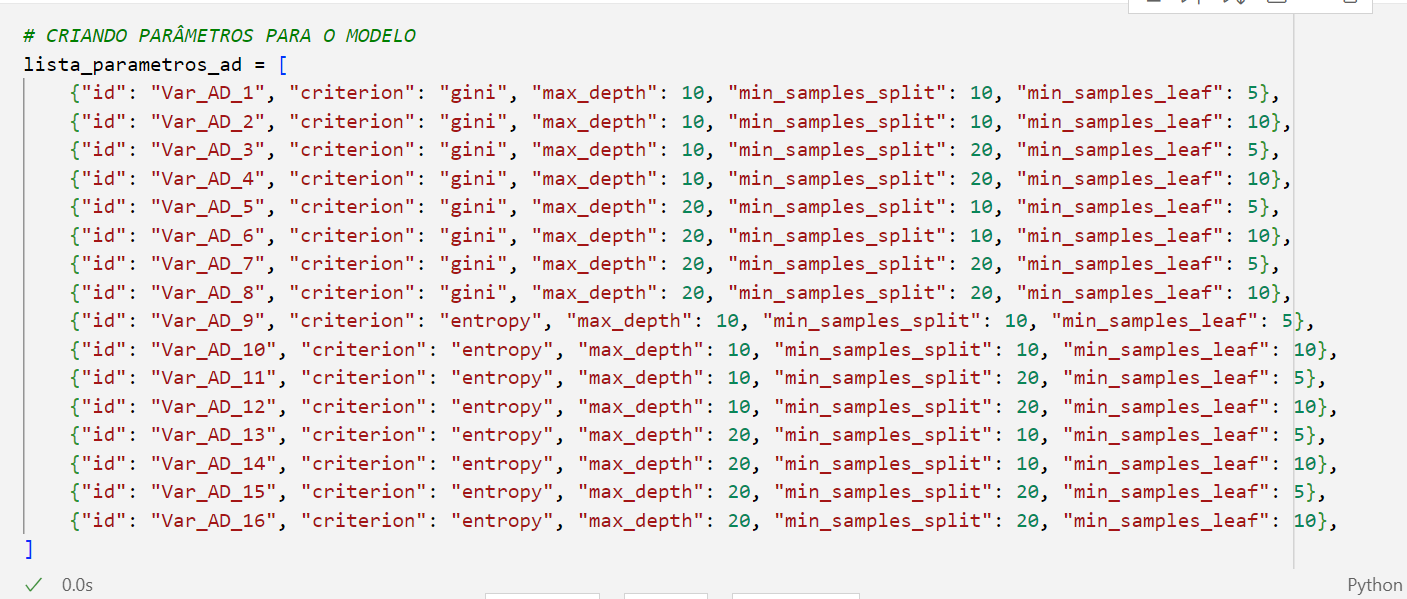
\includegraphics[width=\textwidth]{imagem/adp.png}
\end{center}

\subsection{Performance}

\quad\space Observando os dados armazenados em \textit{lista$\_$resultados$\_$ad} é possível obter:

\begin{center}
	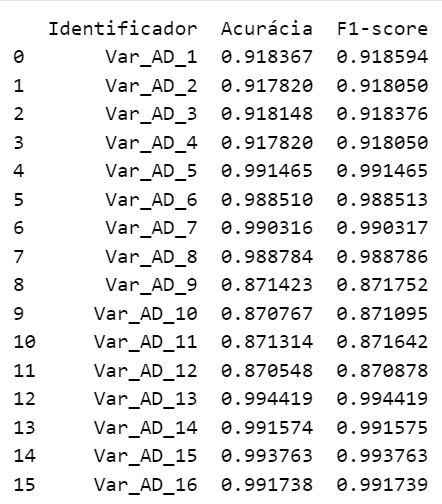
\includegraphics[width=6cm]{imagem/adr.png}
\end{center}

\newpage
\section{Random Forest}
\subsection{Algoritmo utilizado}

\quad\space O algoritmo utilizado para treinar os modelos deste tipo é dado por:

\begin{mdframed}
	\begin{verbatim}
# APLICANDO MODELO
from sklearn.ensemble import RandomForestClassifier
from sklearn.metrics import accuracy_score, f1_score

# criando a lista de resultados finais
lista_resultados_rf = []

for parametros in parametros_rf:
	# criando classificador
	classificador = RandomForestClassifier(
		criterion=parametros["criterion"], 
		max_depth=parametros["max_depth"], 
		min_samples_split=parametros["min_samples_split"], 
		min_samples_leaf=parametros["min_samples_leaf"], 
		n_estimators=100, 
		random_state=42
	)
	
	# treinando o modelo
	classificador.fit(a_treino, r_treino)
	
	# prevendo respostas
	r_previsao = classificador.predict(a_teste)
	
	# calculando métricas
	acuracia = accuracy_score(r_teste, r_previsao)
	f1 = f1_score(r_teste, r_previsao, average="weighted")
	
	# salvando resultados
	lista_resultados_rf.append([parametros["id"], acuracia, f1])
	\end{verbatim}
\end{mdframed}

\vspace{0.5cm}
\subsection{Variações de parâmetros}

\quad\space As variações de parâmetros, em busca da melhor performance, foram:

\begin{center}
	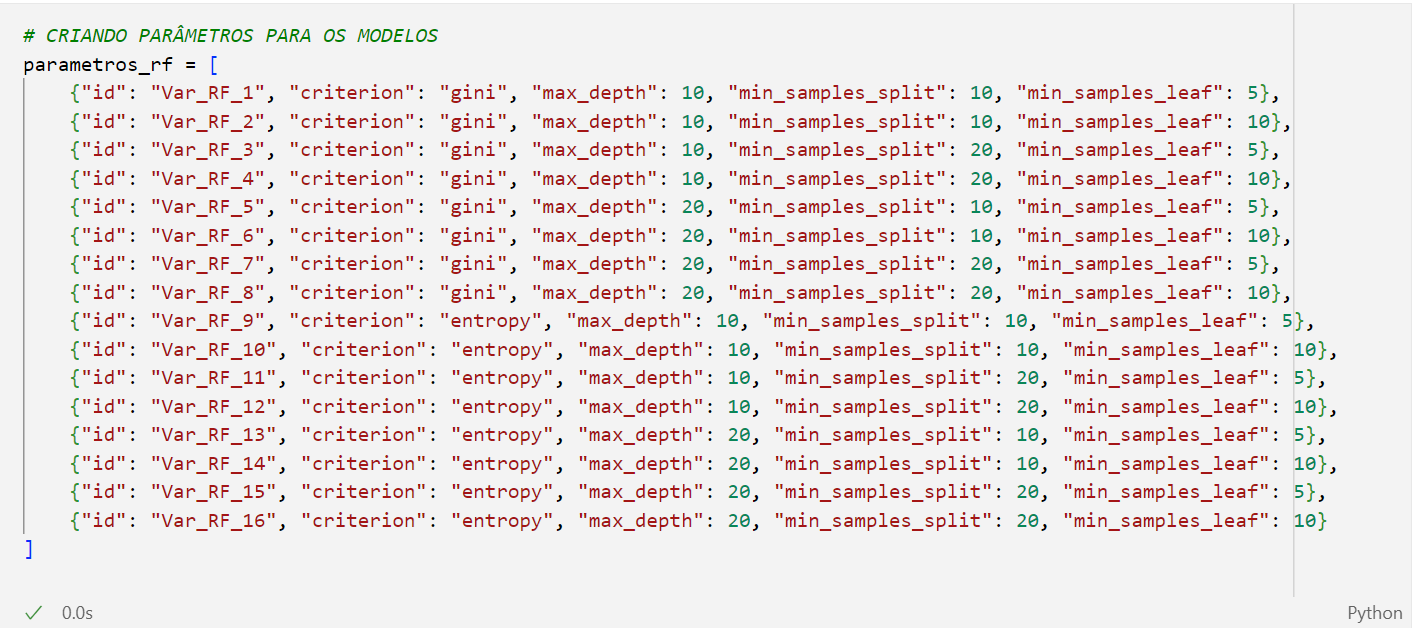
\includegraphics[width=\textwidth]{imagem/rfp.png}
\end{center}

\subsection{Performance}

\quad\space Observando os dados armazenados em \textit{lista$\_$resultados$\_$rf} é possível obter:

\begin{center}
	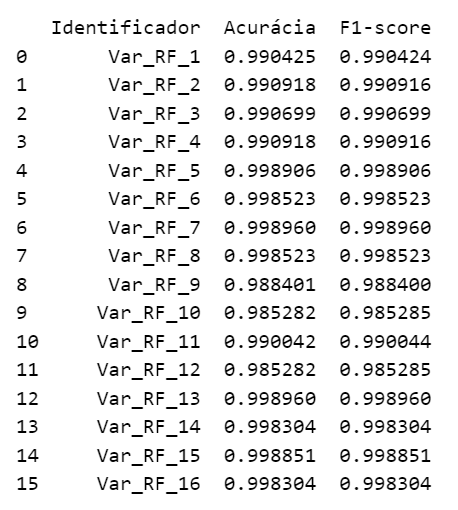
\includegraphics[width=6cm]{imagem/rfr.png}
\end{center}

\newpage
\section{Rede Neural Multilayer Perceptron}

\subsection{Algoritmo utilizado}

\quad\space O algoritmo utilizado para treinar os modelos deste tipo é dado por:

\begin{mdframed}
	\begin{verbatim}
# APLICANDO MODELO
from sklearn.neural_network import MLPClassifier
from sklearn.metrics import accuracy_score, f1_score

# criando a lista de resultados finais
lista_resultados_mlp = []

for parametros in lista_parametros_mlp:
	# criando classificador
	classificador = MLPClassifier(
		hidden_layer_sizes=parametros["hidden_layer_sizes"],
		activation=parametros["activation"],
		max_iter=500,
	)
	
	# treinando o modelo
	classificador.fit(a_treino, r_treino)
	
	# prevendo respostas
	r_previsao = classificador.predict(a_teste)
	
	# calculando métricas
	acuracia = accuracy_score(r_teste, r_previsao)
	f1 = f1_score(r_teste, r_previsao, average="weighted")
	
	# salvando resultados
	lista_resultados_mlp.append([parametros["id"], acuracia, f1])
	\end{verbatim}
\end{mdframed}

\vspace{0.5cm}
\subsection{Variações de parâmetros}

\quad\space As variações de parâmetros, em busca da melhor performance, foram:

\begin{center}
	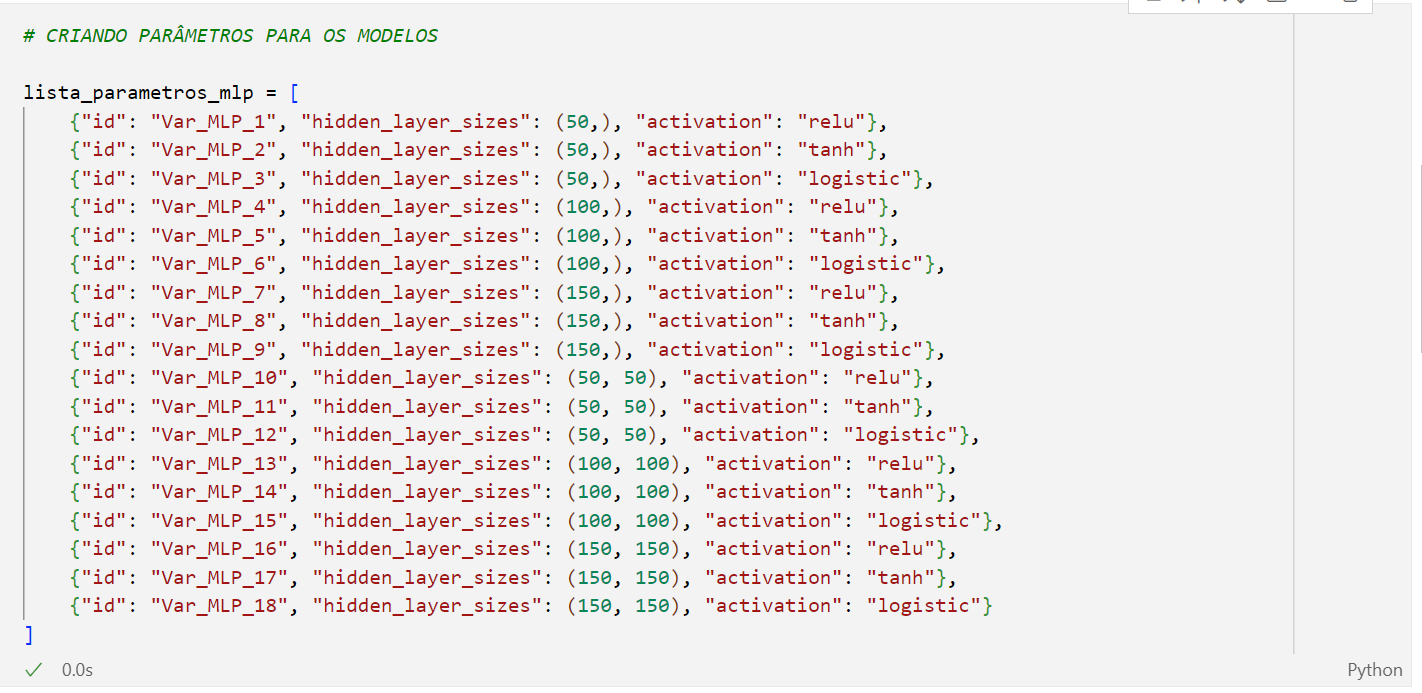
\includegraphics[width=\textwidth]{imagem/mlpp.png}
\end{center}

\subsection{Performance}

\quad\space Observando os dados armazenados em \textit{lista$\_$resultados$\_$mlp} é possível obter:

\begin{center}
	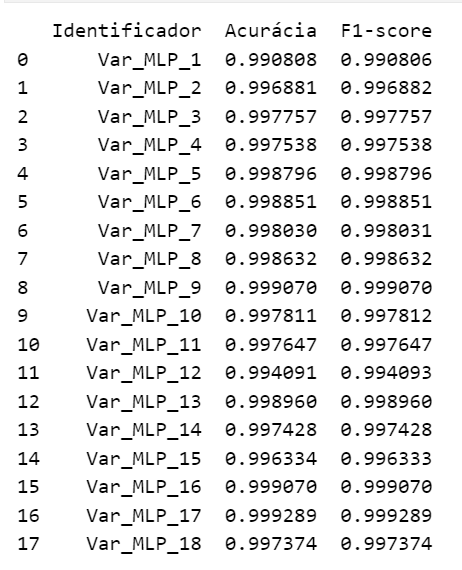
\includegraphics[width=6cm]{imagem/mlpr.png}
\end{center}
\newpage
\section{Conclusão}

\quad\space Observando os modelos de classificação gerados:

\begin{flushleft}
	\textbf{Árvore de Decisão:} o melhor resultado foi obtido com o conjunto de parâmetros \textit{Var$\_$AD$\_$13} (critério de divisão "entropy", profundidade máxima 20, no mínimo 10 amostras necessárias para dividir um nó e no mínimo 5 amostras necessárias para dividir um nó folha) que possui Acurácia e F1-Score de 0.994419.
	
	\vspace{0.5cm}
	\textbf{Random Forest:} o melhor resultado foi obtido nos conjuntos de parâmetros \textit{Var$\_$RF$\_$07} (critério de divisão "gini", profundidade máxima 20, no mínimo 20 amostras necessárias para dividir um nó e no mínimo 5 amostras necessárias para dividir um nó folha) e \textit{Var$\_$RF$\_$13} (critério de divisão "entropy", profundidade máxima 20, no mínimo 10 amostras necessárias para dividir um nó e no mínimo 5 amostras necessárias para dividir um nó folha) quem possuem Acurácia e F1-Score de 0.998960.
	
	\vspace{0.5cm}
	\textbf{Rede Neural Multilayer Perceptron:} o melhor resultado foi obtido com o conjunto de parâmetros \textit{Var$\_$MLP$\_$17} (duas camadas ocultas com 150 neurônios cada e função de ativação "tanh") que possui Acurácia e F1-Score de 0.999289.
	
	\vspace{0.5cm}
	\quad\space Levando em consideração somente as métricas Acurácia e F1-Score, o melhor modelo para colocar em produção dentro do domínio do dataset "Secondary Mushroom" é o modelo \textit{Var$\_$MLP$\_$17} de Rede Neural Multilayer Perceptron. 

	\quad\space Contudo, ao observarmos os tempos médios de execução de cada modelo, é possível perceber que o tipo Multilayer Perceptron apresenta um desempenho mais lento em comparação ao Random Forest e à Árvore de Decisão.


	\begin{table}[h]
		\centering
		\begin{tabular}{|l|l|l|l|}
			\hline
			\textbf{Tipo} & \textbf{Variações} & \textbf{Tempo total} & \textbf{Tempo médio} \\
			\hline
			Árvore de decisão & 16 & 4,7s & 0,29s \\
			\hline
			Random Forest & 16 & 72,5s & 4,53s \\
			\hline
			Multilayer Perceptron & 18 & 846,3s & 47,01s \\
			\hline
		\end{tabular}
	\end{table}
	
	Desta forma, o modelo que apresenta o melhor equilíbrio entre desempenho e tempo de execução é o Random Forest, configurado com os parâmetros \textit{Var$\_$RF$\_$07} ou \textit{Var$\_$RF$\_$13}.
\end{flushleft}

\end{document}
